\section{Context and Motivation}
\label{sec:intro:context}

%Describe the context of activity recognition, enhancing why it is needed and how it has been approached. Explain briefly how knowledge-driven systems work and which are their drawbacks to claim that this dissertation aims at overcoming one of those drawbacks: static activity models.

% Distinguish between activity modelling and recognition; Modelling is not an one-off activity but an iterative multi-phase process; Modelling and recognition are interweaved, both improved incrementally; Add an image where this cycle is shown (Chen's presentation)

Independently from the approach used to implement activity recognition systems, it is usually the case that activity modelling and recognition are carried out separately. Activity modelling is very important for activity recognition, since it provides the models which have to be recognised in the sensor datasets generated by humans while they perform activities. While data-driven approaches obtain those models directly from user generated data, knowledge-driven approaches obtain them by means of knowledge engineering techniques. However, both approaches share usually the same assumption, i.e. activity modelling is performed once and afterwards, the generated models are used for activity recognition. 

% People tend to change the way they perform activities, executing different action sequences for the same activities; this is specially true for elderly people, whose cognitive impairments may be associated with their habit changes

Assuming the static nature of activity models does not fit to the reality. People tend to change the way they perform the same activities in time. Hence, the same activity models cannot be used forever. From the point of view of data-driven activity modelling approaches, implementing dynamic activity models is not a problem, as incremental learning techniques can be used \cite{Rashidi2011}. Moreover, as activity models are learnt directly from user generated data, personalised activity models are naturally obtained. Two of the positive features of data-driven modelling are thus dynamic and personalised models. But those virtues pose also some drawbacks: activity models are not generic so they cannot be applied to other users and activity models are usually incomprehensible for humans which make their usage for other applications much harder.

% Talk about knowledge-driven approaches and show how the activity models obtained by knowledge engineering techniques are usually static; focus specially on actions, which are the key elements for recognition

On the other hand, knowledge-driven modelling produces generic and human understandable models, since activities are modelled by their intrinsic features and relations rather than from data, and activity models are expressed using logical and descriptive formalisms \cite{Chen2012a}. However, those models are usually static, i.e. once they have been defined they do not evolve. In addition to it, obtaining personalised models is very complicated because experts cannot know in advance all the personal features of a concrete user. 

% To have dynamic knowledge-driven activity modelling, a new process is proposed: (i) domain experts provide initial activity models, (ii) inhabitants produce sensor datasets while performing activities, (iii) a learning system improves the initial activity models and presents them to the domain expert, (iv) domain expert validates models and adds them to the knowledge base

It is quite clear then that both activity modelling approaches have complementary advantages and disadvantages. An approach excels where the other fails. It seems natural thus to try to combine both approaches in order to develop a better activity modelling process where generic and personalised models can be obtained and those models evolve in time with user generated data. 

In this dissertation, a continuous activity modelling process is presented, where domain experts provide initially generic activity models using knowledge engineering tools, to afterwards run data-driven learning algorithms on user generated data to learn personalised models. Such personalised models will be presented to the expert, who can add or update them in the knowledge base. This loop is continuously repeated in time to achieve dynamic and personalised models based on initially provided generic models and user generated data. Figure \ref{fig-activity-modelling} shows a diagram with the described process.

\begin{figure}[htbp]
\centering
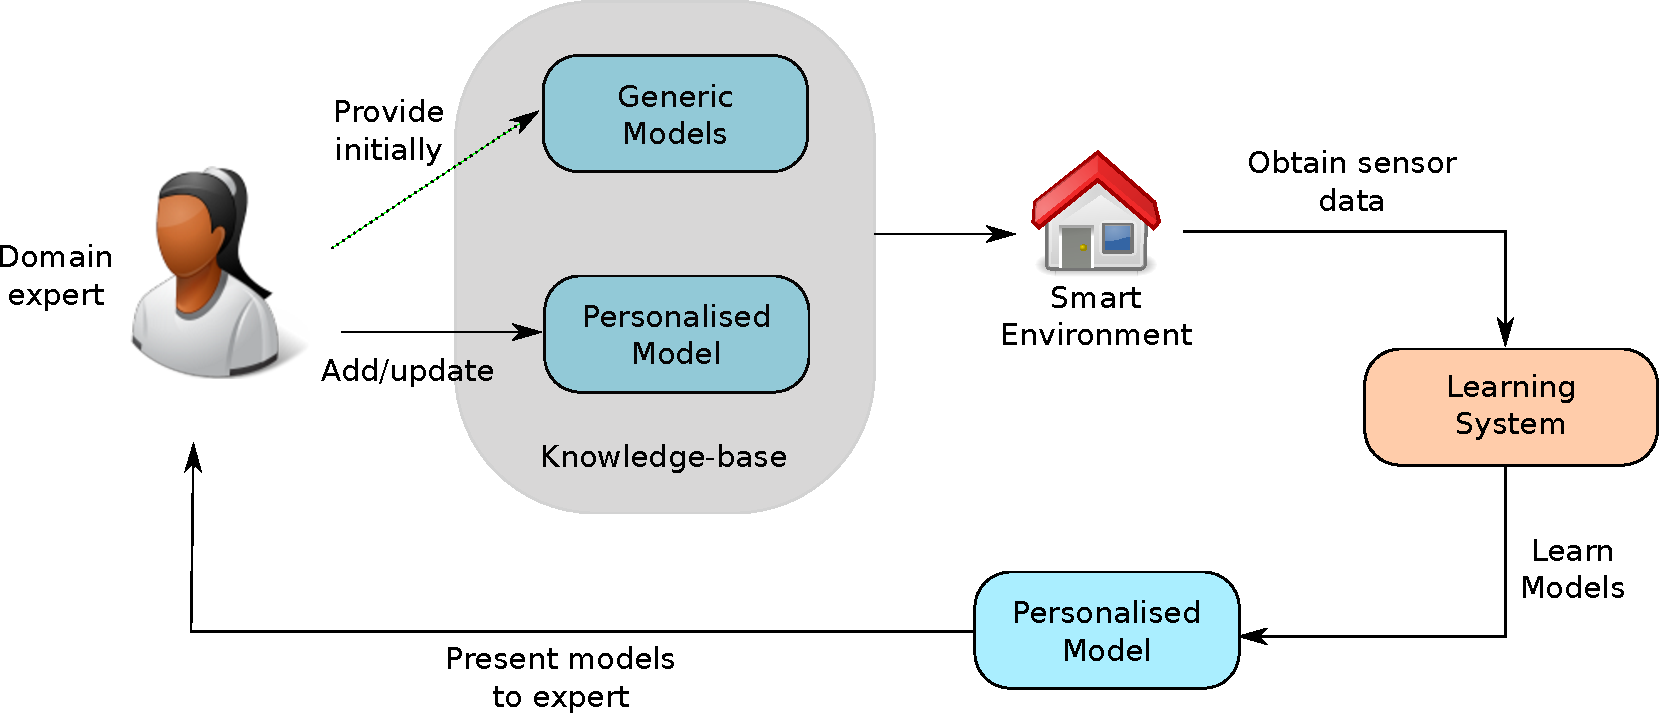
\includegraphics[width=\textwidth]{activity_modelling.pdf}
    \caption{The continuous activity model process to obtain dynamic and personalised models from generic expert provided models.}
    \label{fig-activity-modelling}
\end{figure}

The described activity modelling process uses generic knowledge-based activity models provided by a domain expert, achieving thus generic and understandable activity models. To solve the problem of personalised models, user generated data is used in a learning process to produce knowledge-based personalised models. This means that data-driven learning techniques are used to capture personal features of generic activities and obtain understandable personalised activity models. Such models, after expert validation, are added to the knowledge base to use them subsequently in activity recognition systems. Repeating this process continuously, dynamic activity models are obtained, which evolve in time as users change - or not - their habits.

% One of the key elements of this process is the learning system, which has to learn new actions for already defined activities -> this is the target of the thesis; provide an example (MakeCoffee) with its image

When modelling activities, two major aspects are considered: the actions carried out to perform the activity and the descriptive features of the activity \cite{Chen2014}. Actions refer to object interactions. For example, to prepare a coffee a user might have coffee and a cup to drink the coffee. This sequence can be modelled as the action sequence of \textit{hasCoffee} and \textit{hasContainer}, which are obtained from the interactions with the respective objects monitored by sensors. Descriptive properties of an activity refer to the time when the activity has been performed, its duration, the concrete set of objects used and their order. Both aspects of an activity model, i.e. actions and descriptive properties, may vary from person to person. 

As far as learning personalised descriptive properties for knowledge-based models regards, Chen et al. already combined data-driven and knowledge-driven approaches in \cite{Chen2014}. However, to the best of our knowledge, a similar work to learn specific actions for activity models has not been published yet. In that sense, the work presented in this dissertation tackles a novel problem. In fact, Chen et al. assume in their work that the actions in the \textit{seed} activity models provided by domain experts can be applied to any user. This means that every user has to execute the same actions to perform a concrete activity.

In this dissertation, the problem of learning actions for given activities is analysed. It cannot be generally assumed that every user executes the same actions to perform a concrete activity. Imagine, for instance, that a user prepares a coffee and adds sugar to it. To make it simple, the activity model for this user could contain the actions \textit{hasCoffee}, \textit{hasContainer}, \textit{hasWater} and \textit{hasFlavour}. But there is another user who does not like any flavourant, so she prepares coffee by means of actions \textit{hasCoffee}, \textit{hasContainer} and  \textit{hasWater}. As it can be seen, both activity models are different as far as actions regard, but both of them are valid models for the activity of making a coffee. 

To develop a proper activity modelling process, learning actions is a key feature. It has been observed that generic activity models provided by a domain expert have the necessary actions to perform an activity, but not sufficient actions for personalised models. Those activity models can be used to further learn new actions for different users and thus generate new personalised activity models. Let us illustrate our hybrid activity modelling approach with an example. Figure \ref{fig-objective} shows an initial generic activity model for the MakeCoffee activity, which is composed by the actions \textit{hasCoffee} and \textit{hasContainer}. These are the necessary actions for every person to perform a MakeCoffee activity, which highlight the indispensable actions of making a coffee, i.e. the use of coffee and a container to place the coffee in. Nevertheless, some users might add some milk and sugar, others cream and so on. The idea of our approach is to create high-level activity models with only these indispensable actions - generic models -, and then use the data generated by a specific user performing the activity to learn those new actions which also configure the personal way of making coffee. In the case of Figure \ref{fig-objective}, where the initial activity model will only include coffee and container, the system would learn that MakeCoffee is performed in two ways by the user: in the first one, the user adds milk (\textit{hasMilk}) and sugar (\textit{hasFlavour}), while in the second one only sugar is added (\textit{hasFlavour}). Hence two specialised and complete activity models of MakeCoffee can be learnt. This way, experts, initially, only have to provide generic but incomplete activity models with necessary actions. Afterwards the learning system can analyse a user's behavioural data and learn the specialised and complete models to enrich the knowledge base, thus improving initial activity models.

\begin{figure}[htbp]
\centering
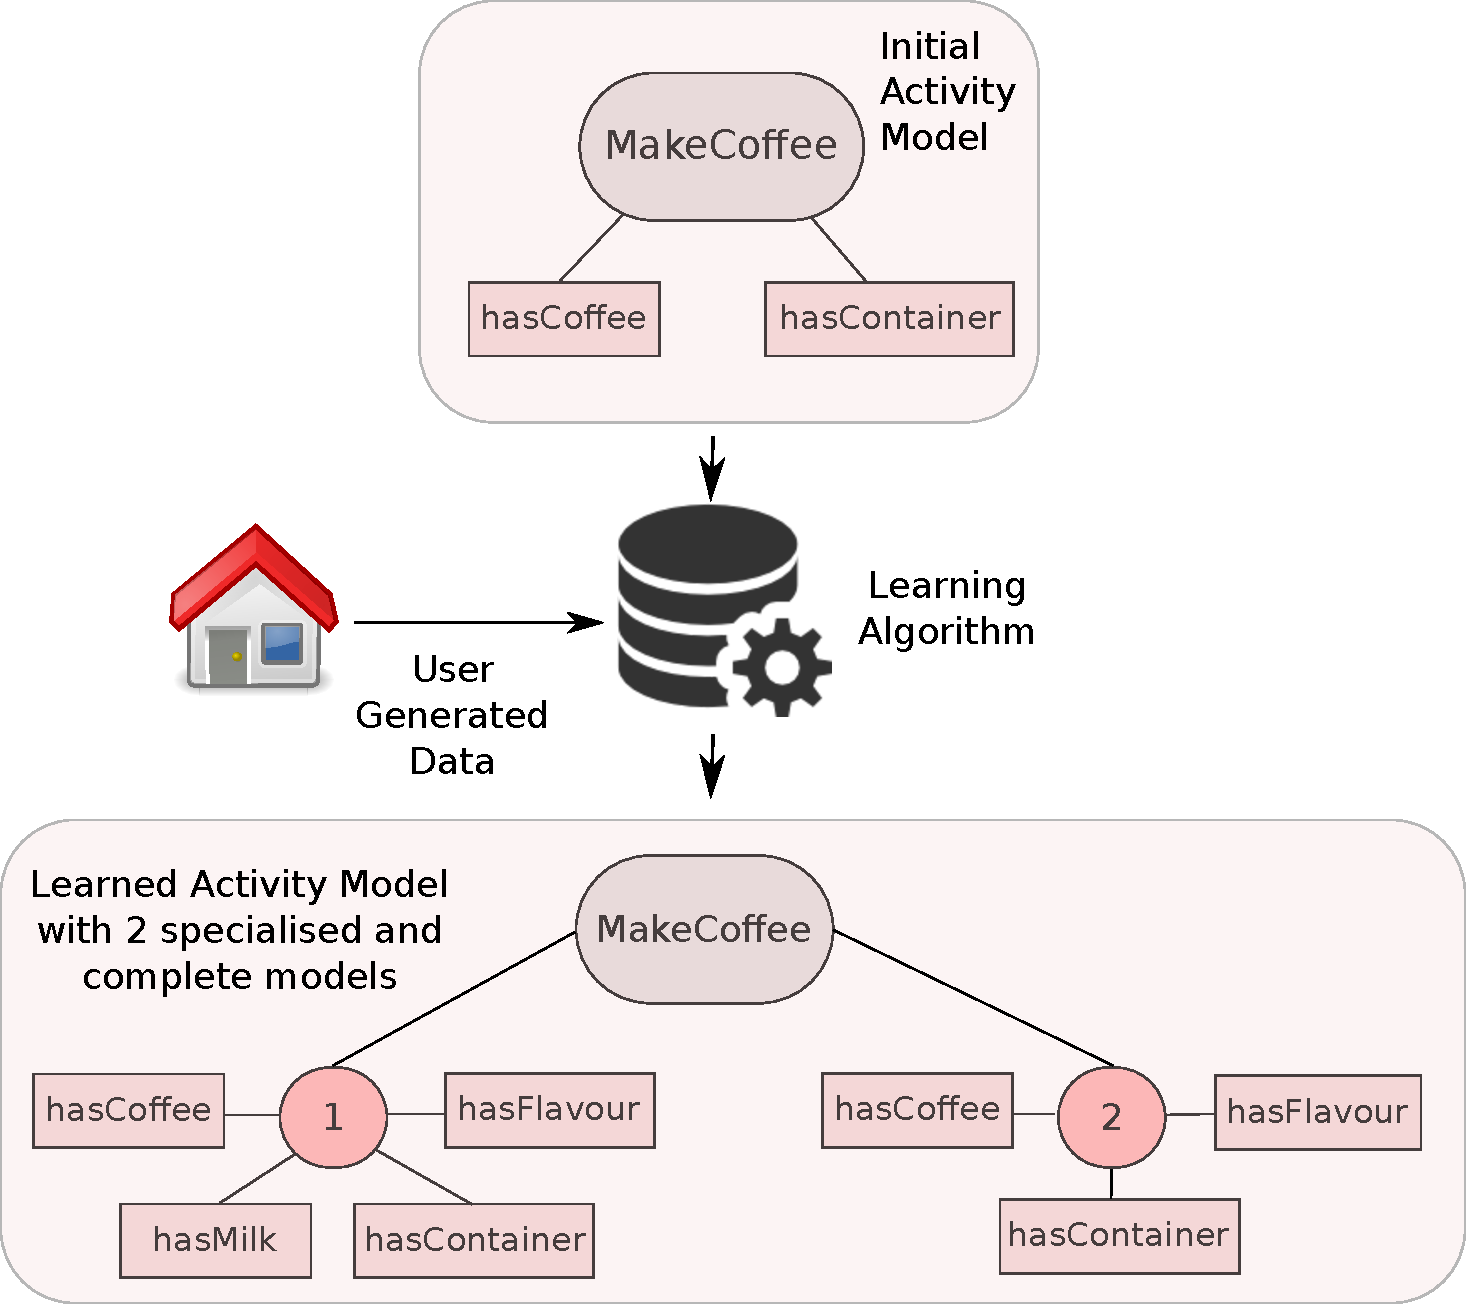
\includegraphics[width=9cm]{objective.pdf}
    \caption{Illustrative example of the objective of the dissertation: using the initial incomplete model for MakeCoffee and user generated data, the learning algorithm learns two specialised and complete models.}
    \label{fig-objective}
\end{figure}


Running the proposed learning process periodically with new data generated by a concrete user, a dynamic activity modelling system is achieved. As a user evolves regarding the way she performs certain activities, the learning approach learns new versions of the initial activity models. Hence, activity models can be adapted to users' varying behaviours.

Notice that the proposed modelling approach does not only learn new actions for initial activity models, but it also learns sub-activities of already defined activities. In the example depicted in Figure \ref{fig-objective}, the two specialised models are two sub-activities of the MakeCoffee activity, namely MakeBlackCoffee and MakeCoffeeWithMilk. This feature makes possible for the expert to define activities in a higher level of abstraction and let the system learn different sub-activities to generate specialised knowledge. 

As a summary, this dissertation is focused on making another step towards dynamic and personalised activity models for knowledge-driven activity recognition systems. A learning system to obtain complete and specialised activity models from generic but incomplete expert provided models has been developed. This step allows implementing activity modelling approaches that use expert knowledge to have generic activity models applicable to every user, and learn new actions for concrete users achieving personalised and dynamic activity models. 